% Quiz 02 --- Small-world networks. Printed, worked in class, 15 minutes.
%
% The sheet carries the questions only. No boxes and no ruled lines: students
% write on the back or on their own paper, and the Google Form takes a photo.
%
% Compile with: xelatex -interaction=nonstopmode quiz02.tex   (run twice)
\documentclass[a4paper, 12pt]{extarticle}
% Shared preamble for Quiz 02 (quiz02.tex and solutions.tex).
% Compile with: xelatex -interaction=nonstopmode <file>.tex   (run twice)
%
% Same house look as the pen-and-paper sheets in
% lecture-note/*/pen-and-paper/: Charter, A4, generous leading, room to draw.

\usepackage[top=0.7in, bottom=0.6in, left=0.8in, right=0.8in]{geometry}
\usepackage{amsmath}
\usepackage{amssymb}
\usepackage{array}
\usepackage{graphicx}
\usepackage[hidelinks]{hyperref}
\usepackage{tcolorbox}
\usepackage{enumitem}
\usepackage{etoolbox}
\usepackage{tikz}
\usepackage{fontspec}
\usetikzlibrary{calc,positioning,arrows.meta}
\definecolor{pltblue}{HTML}{1F77B4}
\definecolor{rulegrey}{HTML}{6A6D75}

% Body face. Charter, and the four ways to get it. XCharter *is* Charter and
% ships with a full TeX Live, so it is asked for first and by file: a CI runner
% answers yes to \IfFontExistsTF{Charter}, then cannot typeset it.
\IfFontExistsTF{XCharter-Roman.otf}{
  \setmainfont{XCharter}[
    Extension      = .otf,
    UprightFont    = *-Roman,
    BoldFont       = *-Bold,
    ItalicFont     = *-Italic,
    BoldItalicFont = *-BoldItalic]
}{
  \IfFontExistsTF{Charter}{\setmainfont{Charter}}{
    \IfFontExistsTF{Iowan Old Style}{\setmainfont{Iowan Old Style}}{
      \IfFontExistsTF{Georgia}{\setmainfont{Georgia}}{}}}}

\setlength{\parindent}{0pt}
\setlength{\parskip}{0.4em}
\setlength{\emergencystretch}{1.2em}
\raggedbottom
\pagestyle{empty}

% ---------------------------------------------------------------------------
% The submission link.
%
% Both the QR square and the printed address are the course's own short link,
% not the form's: paper outlives any one form. Caddy on the course droplet
% points go.skojaku.com/ans-quiz02 at the current Google Form
% (/etc/caddy/Caddyfile, block go.skojaku.com). Swapping the form is a line on
% the server, not a reprint.
%
% If the link ever changes, rebuild the square with
%
%   uvx --from segno segno --output=quiz02-form-qr.png --scale=20 --border=1 \
%       --error=m "<the url>"
%
% PNG rather than PDF for the square: segno's PDF is too spare for xdvipdfmx to
% include, and a QR is squares, so 700px across a 3cm box is already sharper
% than the printer.
% ---------------------------------------------------------------------------
\newcommand{\formlink}{https://go.skojaku.com/ans-quiz02}
\newcommand{\formshort}{\href{\formlink}{\texttt{go.skojaku.com/ans-quiz02}}}

% Quiz header. #1 = title, #2 = the line under it, #3 = term.
\newcommand{\quizhead}[3]{%
  {\footnotesize\textsc{Advanced Network Science} \hfill \textsc{#3}}\par
  \vspace{-0.2em}\rule{\textwidth}{1pt}\par
  \vspace{0.3em}
  {\LARGE\bfseries #1}\par
  \vspace{0.1em}
  {\small #2}\par
  \vspace{0.7em}
  {\small Name \underline{\hspace{6cm}} \hfill Date \underline{\hspace{3.2cm}}}\par
  \vspace{0.7em}}

% A question heading with its point value.
\newcommand{\question}[3]{%
  \vspace{0.5em}
  {\large\bfseries Question #1 \quad\normalsize\mdseries (#2 points)}\par
  \vspace{-0.3em}{\color{rulegrey}\rule{\textwidth}{0.6pt}}\par
  \vspace{0.1em}
  {\bfseries #3}\par
  \vspace{0.2em}}

% An empty box to draw or write in. #1 = height, #2 = caption under the rule.
\newcommand{\drawbox}[2]{%
  \begin{tcolorbox}[colback=white, colframe=rulegrey, boxrule=0.5pt,
                    sharp corners, height=#1, valign=top,
                    boxsep=2pt, left=4pt, right=4pt, top=3pt, bottom=3pt]
  {\footnotesize\color{rulegrey} #2}
  \end{tcolorbox}}

% Ruled writing lines, #1 of them.
\newcommand{\writelines}[1]{%
  \vspace{0.3em}
  \foreach \i in {1,...,#1}{%
    {\color{rulegrey}\rule{\textwidth}{0.4pt}}\par\vspace{1.5em}}}


\tikzset{
  gnode/.style={circle, draw=pltblue, fill=pltblue!12, line width=0.9pt,
                minimum size=7mm, inner sep=0pt, font=\small\bfseries},
  gedge/.style={line width=0.9pt, draw=rulegrey}
}

\begin{document}

\quizhead{Quiz 2 \; --- \; Small-world networks}
        {15 minutes \quad$\cdot$\quad 10 points \quad$\cdot$\quad
         Closed notes, work on your own}
        {Fall 2026}

\begin{tcolorbox}[colback=white, colframe=rulegrey, boxrule=0.5pt,
                  sharp corners, boxsep=1pt, top=4pt, bottom=4pt]
\begin{minipage}[c]{0.19\textwidth}
\begin{center}

\includegraphics[width=2.2cm]{quiz02-form-qr.png}
\end{center}
\end{minipage}
\hfill
\begin{minipage}[c]{0.77\textwidth}
{\small
\textbf{You hand in two photos, one per question.}
Write each question's answer
on its own page. Then photograph each page and upload it.

\vspace{0.2em}

Point a camera at the square, or type \formshort.
}
\end{minipage}
\end{tcolorbox}

% ---------------------------------------------------------------------------
\question{1}{6}{Measure this network.}

\vspace{-1.1em}
\begin{center}
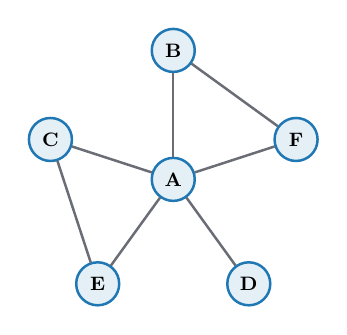
\begin{tikzpicture}[scale=0.78, every node/.style={transform shape}]
  \node[gnode] (A) at ( 0.00,  0.00) {A};
  \node[gnode] (B) at ( 0.00,  2.10) {B};
  \node[gnode] (F) at ( 2.00,  0.65) {F};
  \node[gnode] (D) at ( 1.23, -1.70) {D};
  \node[gnode] (E) at (-1.23, -1.70) {E};
  \node[gnode] (C) at (-2.00,  0.65) {C};
  \draw[gedge] (A) -- (B);
  \draw[gedge] (A) -- (C);
  \draw[gedge] (A) -- (D);
  \draw[gedge] (A) -- (E);
  \draw[gedge] (A) -- (F);
  \draw[gedge] (B) -- (F);
  \draw[gedge] (C) -- (E);
\end{tikzpicture}
\end{center}
\vspace{-1.1em}

\textbf{(a) [3 pts]} Compute the \textbf{global clustering coefficient}
\[
  C \;=\; \frac{3 \times (\text{number of triangles})}
                {\text{number of connected triples}},
\]
where a \emph{connected triple} is a node together with an unordered pair of
its neighbors. Give the two counts before you give $C$.

\vspace{0.1em}

\textbf{(b) [3 pts]} Compute the \textbf{average path length} $\langle \ell
\rangle$: the mean shortest-path distance over all $\binom{6}{2}$ unordered
pairs of distinct nodes. Show how the pairs split by distance before you give
the average.

% ---------------------------------------------------------------------------
\question{2}{4}{A tempting index.}

Suppose we define the \emph{small-worldness} of a network as the ratio of the
two numbers you just computed,
\[
  S \;=\; \frac{C}{\langle \ell \rangle}.
\]
A network is then called ``more small-world'' the larger $S$ is.

\vspace{0.2em}

\textbf{(a) [2 pts]} This definition is broken. Say what is wrong with a concrete case, e.g., two networks that $S$ ranks the wrong
way round.

\vspace{0.2em}

\textbf{(b) [2 pts]} Repair it. Write down a definition that does not have the
problem you named. Why does this address the problem?

\vfill

\end{document}
